\section{\textbf{Addressing Dependencies in Dyadic Data}}

Relational, or dyadic, data structures provide measurements of how pairs of actors relate to one another. These structures encompass events of interest as diverse as the level of trade between $i$ and $j$ to the occurrence of an interstate conflict. The easiest way to organize such data is the directed dyadic design in which the unit of analysis is some set of $n$ actors that have been paired together to form a dataset of $z$ directed dyads. A tabular design such as this for a set of $n$ actors, $\{i, j, k, l \}$ results in $n \times (n-1)$ observations, as shown in Table~\ref{tab:canDesign}. 

\begin{table}[ht]
	\captionsetup{justification=raggedright }
	\centering
	\begin{minipage}{.45\textwidth}
		\centering
		\begingroup
		\setlength{\tabcolsep}{10pt}
		\begin{tabular}{ccc}
			Sender & Receiver & Event \\
			\hline\hline
			$i$ & $j$ & $y_{ij}$ \\
			\multirow{2}{*}{\vdots} & $k$ & $y_{ik}$ \\
			~ & $l$ & $y_{il}$ \\
			$j$ & $i$ & $y_{ji}$ \\
			\multirow{2}{*}{\vdots} & $k$ & $y_{jk}$ \\
			~ & $l$ & $y_{jl}$ \\
			$k$ & $i$ & $y_{ki}$ \\
			\multirow{2}{*}{\vdots} & $j$ & $y_{kj}$ \\
			~ & $l$ & $y_{kl}$ \\
			$l$ & $i$ & $y_{li}$ \\
			\multirow{2}{*}{\vdots} & $j$ & $y_{lj}$ \\
			~ & $k$ & $y_{lk}$ \\
			\hline\hline
		\end{tabular}
		\endgroup
		\caption{Structure of datasets used in canonical design.} 
		\label{tab:canDesign}
	\end{minipage}
	$\mathbf{\longrightarrow}$
	\begin{minipage}{.45\textwidth}
		\centering
		\begingroup
		\setlength{\tabcolsep}{10pt}
		\renewcommand{\arraystretch}{1.5}
		\begin{tabular}{c||cccc}
		~ & $i$ & $j$ & $k$ & $l$ \\ \hline\hline
		$i$ & \footnotesize{NA} & $y_{ij}$ & $y_{ik}$ & $y_{il}$ \\
		$j$ & $y_{ji}$ & \footnotesize{NA}  & $y_{jk}$ & $y_{jl}$ \\
		$k$ & $y_{ki}$ & $y_{kj}$ & \footnotesize{NA}  & $y_{kl}$ \\
		$l$ & $y_{li}$ & $y_{lj}$ & $y_{lk}$ & \footnotesize{NA}  \\
		\end{tabular}
		\endgroup
		\caption{Adjacency matrix representation of data in Table~\ref{tab:canDesign}. Senders are represented in the rows and receivers the columns. }
		\label{tab:netDesign}
	\end{minipage}
\end{table}

\subsection{Limitations of the Standard Framework}

When modeling these types of data structures, scholars typically employ a generalized linear model (GLM) estimated via maximum-likelihood. This type of model can be expressed via a stochastic and systematic component \citep{pawitan:2013}. The stochastic component reflects our assumptions about the probability distribution from which the data is generated: $y_{ij} \simiid \mathcal{F}(\theta_{ij})$, where $\mathcal{F}$ represents a probability distribution or mass function such as normal or binomial, and $\simiid$ represents the assumption that each dyad in our sample is independently drawn from that particular distribution. The systematic component characterizes the model for the parameters of that distribution and describes how $\theta_{ij}$ varies as a function of a set of nodal and dyadic covariates, $\mathbf{X}_{ij}$: $\theta_{ij} = \bm\beta^{T} \mathbf{X}_{ij}$. A fundamental assumption we make when applying this modeling technique is that given $\mathbf{X}_{ij}$ and the parameters of our distribution, each of the dyadic observations is conditionally independent. 

The import of this assumption becomes clearer in the process of estimating a GLM via maximum likelihood. After having chosen a set of covariates and specifying a distribution, we construct joint density function over all dyads.

\begin{align}
\begin{aligned}
	Pr(y_{ij}, y_{ik}, \ldots, y_{lk} | \theta_{ij}, \theta_{ik}, \ldots, \theta_{lk}) &= \mathcal{F}(\theta_{ij}) \times \mathcal{F}(\theta_{ik}) \times \ldots \times \mathcal{F}(\theta_{lk}) \\
	Pr(\mathbf{Y}=(y_{ij}, y_{ik}, \ldots, y_{lk}) \; | \; \bm{\theta}=(\theta_{ij}, \theta_{ik}, \ldots, \theta_{lk})) &= \prod_{a=1}^{z} \mathcal{F}(\theta_{a})  \\
\end{aligned}
\end{align}

We next convert the joint probability into a likelihood by assuming the observations are fixed but the distributional parameters, $\bm{\theta}$, are assumed to be random:%\footnote{For further discussion see \citet{pawitan:2013} or other introductory sources to maximum-likelihood estimation.}

\begin{align}
\begin{aligned}
	\mathcal{L} (\bm{\theta} | \mathbf{Y}) &= k(\mathbf{Y}) \times Pr(\mathbf{Y} | \bm{\theta}) \\
	\mathcal{L} (\bm{\theta} | \mathbf{Y}) &= k(\mathbf{Y}) \times \prod_{a=1}^{z} \mathcal{F}(y_{a} | \theta_{a}) \\	
	\mathcal{L} (\bm{\theta} | \mathbf{Y}) &\propto \prod_{a=1}^{z} \mathcal{F}(y_{a} | \theta_{a}) \\
\end{aligned}
\end{align}

This likelihood   can be solved through maximization or numerical analysis. However, the important point to note is that the likelihood as defined above is only valid if we are able to make the assumption that, for example, $y_{ij}$ is independent of $y_{ji}$ and $y_{ik}$ given the set of covariates we specified.\footnote{The difficulties of applying the GLM framework to data structures that have structural interdependencies between observations is a problem that has long been recognized. \citet{beck:katz:1995}, for example, detail the issues with pooling observations in time-series cross-section datasets. \citet{ward:gleditsch:2008} have done the same in the case of spatial dependence.} Assuming that the dyad $y_{ij}$ is independent of the dyad $y_{ji}$ asserts that there is no level of reciprocity in a dataset, an assumption that in many cases would seem quite untenable.\footnote{For example, see \citet{ward:etal:2007,cranmer:2014,dorff:minhas:2016}.} A harder problem to handle is the assumption that $y_{ij}$ is independent of $y_{ik}$, the difficulty here follows from the possibility that $i$'s relationship with $k$ is dependent on how $i$ relates to $j$ and how $j$ relates to $k$, or more simply put the ``enemy of my enemy [may be] my friend''. 

The presence of these types of interdependencies in relational data structures is exactly why we are interested in the, but complicates the a priori assumption of observational independence. Without this assumption the joint density function cannot be written in the way described above and  a valid likelihood does not exist.\footnote{This problem has been noted in works such as \citet{lai:1995,manger:etal:2012,kinne:2013}.} Accordingly inferences drawn from misspecified models that ignore potential interdependencies between dyadic observations are likely to have a number of issues including biased estimates of the effect of independent variables, uncalibrated confidence intervals, and poor predictive performance. Just as important, however, is that by ignoring these interdependencies we ignore a potentially important part of the data generating process behind relational data structures, namely, network phenomena. 

\subsection{Social Relations Model: Additive Part of AMEN}

The dependencies that tend to develop in relational data can be more easily understood when we move away from stacking dyads on top of one another and turn instead to adjacency matrices as shown in Table~\ref{tab:netDesign}. Operationally, this type of data structure is represented as a $n \times n$ matrix, $\mathbf{Y}$, where the diagonals in the matrix are typically undefined.\footnote{Most of the relational variables studied in political science do not involve events that countries can send to themselves.} The $ij^{th}$ entry defines the relationship between $i$ and $j$ and can be continuous or discrete. If the matrix is undirected, the $ji^{th}$ entry will equal the $ij^{th}$ entry. For example, in undirected event data an event cannot be attributed to a specific sender or receiver rather it is just an indication of something that happened between a pair of countries. An example  that commonly arises in the IR literature involves models of alliance relationships: two countries are allied. In directed matrices, the off-diagonal values are not symmetric and there is a clear sender and receiver as in the case of bi-lateral trade or multilateral aid.  

A common type of structural interdependency that arises in relational data structures is ``preferential attachment'' \citep{barabasi:reka:1999,reka:etal:1999}. This is typically categorized as a first-order, or nodal, dependency and represents the fact that we typically find significant heterogeneity in activity levels across nodes. The implication of this across-node heterogeneity is within-node heterogeneity of ties, meaning that values across a row, say $\{y_{ij},y_{ik},y_{il}\}$, will be more similar to each other than other values in the adjacency matrix because each of these values has a common sender $i$. This type of dependency manifests in cases where sender $i$ tends to be more active in the network than other senders. The emergence of this type of structure often occurs in relational datasets such as trade and conflict. In both these cases, there are a set of countries that tend to be more active than others. Similarly, while some actors may be more active in sending ties to others in the network, we might also observe that others are more popular targets, this would manifest in observations down a column, $\{y_{ji},y_{ki},y_{li}\}$, being more similar. Last, we might also find that actors who more likely to send ties in a network are also more likely to receive them, meaning that the row and column means of an adjacency matrix may be correlated. First-order dependencies are equally important to take into account in undirected relational structures, the only difference being that nodal heterogeneity will be equivalent across rows and columns. The presence of this type of heterogeneity in directed and undirected relational data structures leads to a violation of the conditional independence assumption underlying the models in our standard tool-kit.\footnote{It can lead to so-called power law dynamics, which has reinforced the popularity of the assumption of preferential attachment in network studies.}

Another ubiquitous type of structural interdependency is reciprocity. This is a second-order, or dyadic, dependency relevant only to directed datasets, and asserts that values of $y_{ij}$ and $y_{ji}$ may be statistically dependent. In studies of social and economic behavior, direct reciprocity -- the notion that actors learn to ``respond in kind" to one another -- is argued to be an essential component of behavior.\footnote{For example, see \cite{bolton:1998, cox:2007}.} More specifically, this concept actually has deep roots in political science theories of cooperation and the evolution of norms between states \citep{richardson:1960,choucri:north:1972,keohane:1989,rajmaira:ward:1990,goldstein:freem:1990,goldstein:freeman:1991,ward:rajmair:1992,brandt:etal:2008}.  The clearest example of the relevance of this dependency comes from the conflict literature, as we would expect that if, for instance, Iran behaved aggressively towards Saudi Arabia that this would induce Saudi Arabia to behave aggressively in return. The prevalence of these types of potential interactions within directed dyadic data structures also complicates the basic assumption of observational independence.

The relevance of modeling first- and second-order dependencies has long been recognized within some social sciences such as psychology. citet{warner:etal:1979} developed the social relational model (SRM), a type of ANOVA decomposition technique, that facilitates this undertaking.\footnote{\citet{dorff:ward:2013} provide an introduction to this model and \citet{dorff:minhas:2016} apply this approach to studying reciprocal behavior in economic sanctions.} The SRM is of particular note as it provides the error structure for the additive effects component of the AMEN framework that we introduce here. The goal of the SRM is to decompose the variance of observations in an adjacency matrix in terms of heterogeneity across row means (out-degree), heterogeneity along column means (in-degree), correlation between row and column means, and correlations within dyads. \citet{wong:1982} and \citet{li:loken:2002} provide a random effects representation of the SRM:

\begin{align}
\begin{aligned}
	y_{ij} &= \mu + e_{ij} \\
	e_{ij} &= a_{i} + b_{j} + \epsilon_{ij} \\
	\{ (a_{1}, b_{1}), \ldots, (a_{n}, b_{n}) \} &\simiid N(0,\Sigma_{ab}) \\ 
	\{ (\epsilon_{ij}, \epsilon_{ji}) : \; i \neq j\} &\simiid N(0,\Sigma_{\epsilon}), \text{ where } \\
	\Sigma_{ab} = \begin{pmatrix} \sigma_{a}^{2} & \sigma_{ab} \\ \sigma_{ab} & \sigma_{b}^2   \end{pmatrix} \;\;\;\;\; &\Sigma_{\epsilon} = \sigma_{\epsilon}^{2} \begin{pmatrix} 1 & \rho \\ \rho & 1  \end{pmatrix}
\label{eqn:srmCov}
\end{aligned}
\end{align}

The basic idea here is quite simple, $\mu$ provides a baseline measure of the density or sparsity of a network, and $e_{ij}$ represents residual variation. We then decompose that residual variation into parts, namely, a row/sender effect ($a_{i}$), a column/receiver effect ($b_{j}$), and a within dyad effect ($\epsilon_{ij}$). The row and column effects are modeled jointly to account for correlation in how active an actor is in sending and receiving ties. Heterogeneity in the row and column means is captured by $\sigma_{a}^{2}$ and $\sigma_{b}^{2}$, respectively, and $\sigma_{ab}$ describes the linear relationship between these two effects (i.e., whether actors who send [receive] a lot of ties also receive [send] a lot of ties). Beyond these first-order dependencies, variation across second-order dependencies is described by $\sigma_{\epsilon}^{2}$ and a within dyad correlation, or reciprocity, parameter $\rho$. 

\citet{hoff:2005} shows that the SRM covariance structure described in Equation~\ref{eqn:srmCov} can be incorporated into the systematic component of a GLM framework to produce a generalized (bi-)linear mixed effects model: $\bm\beta^{T} \mathbf{X}_{ij} + a_{i} + b_{j} + \epsilon_{ij}$, where $ \bm\beta^{T} \mathbf{X}_{ij}$ accommodates the inclusion of dyadic, sender, and receiver covariates. This approach  effectively incorporates row, column, and within-dyad dependence in way that is widely used and understood by applied researchers: a regression framework. Further this approach can be extended to a handle a diversity of outcome distributions (e.g., binomial, ordinal, etc.). In the case of binary data this can be done by utilizing a latent variable representation of a probit regression model. Specifically, we model a latent variable, $\theta_{ij}$, with a linear predictor and we model the error using the SRM from Equation~\ref{eqn:srmCov}: $\theta_{ij} = \bm\beta^{T} \mathbf{X}_{ij} + e_{ij}$. Then we can simply utilize a threshold model linking $\theta_{ij}$ to our observed values of $y_{ij}$, in the case of a binomial outcome distribution the threshold model can be expressed as: $y_{ij} = I(\theta_{ij}>0)$.  It can also easily incorporate ordinal and rank ordered data.

% The result is actually a model that is very similar to the p1 and p2 ERGMs developed by \citet{holland:leinhardt1981} and \citet{duijn:etal:2004}, respectively. 

\subsection{Latent Factor Model: Multiplicative Part of AMEN}

Missing from the framework provided by the SRM is an accounting of third order dependence patterns that can arise in relational data. The ubiquity of third order effects in relational datasets arises from the presence of some set of shared attributes between nodes that affects their probability of interacting with one another. For example, one finding form the gravity model of trade is that neighboring countries are more likely to trade with one another, in this case, the shared attribute is simply geographic proximity. A finding common in the political economy literature is that democracies are more likely to form trade agreements with one another, and the shared attribute here is a country's political system. Both geographic proximity and a country's political system are examples of homophily, which captures the idea that the relationships between actors with similar characteristics in a network are likely to be stronger than nodes with varying characteristics.\footnote{Homophily can be used to explain the emergence of patterns such as transitivity (``a friend of a friend is a friend'') and balance (``an enemy of a friend is an enemy''). See \citet{shalizi:thomas:2011} for a more detailed discussion on the concept of homophily.} 

More generally, say that we have a binary network where actors tend to form ties to others based on some set of shared characteristics. This often leads to a network graph with a high number of ``transitive triplets'', that is cases in which we have sets of actors $\{i,j,k\}$ each being linked to one another. The left-most plot in figure~\ref{fig:homphStochEquivNet} provides a representation of a network that exhibits this type of pattern. Structures such as this can develop when the interactions between actors results from some set of shared attributes those actors may possess (e.g., they are neighbors of one another, part of an alliance agreement, share similar political systems). The relevant implication of this when it comes to conducting statistical inference is that--unless we are able to specify the list of exogenous variable that may explain homophily--the probability of $j$ and $k$ forming a tie is neither independent of the ties that already exist between those actors and $i$, nor higher than the probability that either of those actors might form a tie with another actor, $l$ with whom they have no shared attributes. 

\begin{figure}[ht]
	\centering
	\begin{tabular}{lcr}
	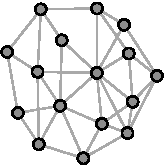
\includegraphics[width=.4\textwidth]{homophNet} & \hspace{2cm} &
	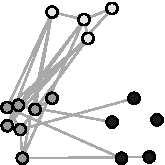
\includegraphics[width=.4\textwidth]{stochEquivNet}	
	\end{tabular}
	\caption{Graph on the left is a representation of an undirected network that exhibits a high degree of homophily, while on the left we show an undirected network that exhibits stochastic equivalence. }
	\label{fig:homphStochEquivNet}
\end{figure}

Another third-order dependence pattern that cannot be accounted for in the additive effects framework discussed in the previous section is stochastic equivalence. A pair of actors $ij$ are stochastically equivalent if the probability of $i$ relating to, and being related to, by every other actor is the same as the probability for $j$ \citep{anderson:etal:1992}. More simply put this refers to the idea that there will be groups of nodes in a network with similar relational patterns. The occurrence of a dependence pattern such as this is not uncommon in the social sciences. \citet{manger:etal:2012} posit and estimate a stochastic equivalence structure to explain the formation of preferential trade agreements (PTAs). Specifically, they suggest that PTA formation is related to differences in per capita income levels between countries. Countries falling into high, middle, and low income per capita levels will have patterns of PTA formation that are determined by the groups into which they fall. They find that PTA formation occurs with greater probability in the following order high-middle, high-high, and middle-middle income groups, and that low income countries are rather unlikely to form PTAs with any partner. Such a structure is represented in the right-most panel of Figure~\ref{fig:homphStochEquivNet}, here the lightly shaded group of nodes at the top can represent high-income countries, nodes on the bottom-left middle-income, and the darkest shade of nodes low-income countries. The main point is that the behavior of actors in a network can at times be governed by group level dynamics, Failing to account for such patterns misleads in that it discounts or completely ignores an important part of the underlying data generating process that is the focus of inquiry. 

If we are able to explicitly model the variety of shared attributes that might cause third-order dependence patterns to develop, then the additive effects described above  justifies the conditional independence assumption that is central to the GLM framework we introduced earlier. The \pkg{amen} package even provides for the estimation of that type of model using a Bayesian framework.\footnote{The main function in the \pkg{amen} package is titled ``ame'' and by default it runs a model assuming that no multiplicative effects are necessary.} There is also a set of utilities one can use to determine whether the inclusion of multiplicative effects is necessary, we will review these in the application section. In the context of most observational research, however, this assumption is untenable. The implausibility of this assumption is manifest.
%, in spirit, the same reason why we no longer model time-series cross-sectional data without including country level fixed or random effects.

\subsubsection{\textbf{ERGMs}}

Within political science the two most often used approaches to accounting for third order dependencies in relational data are ERGMs and latent space models. Exponential Random Graph Models were first developed by \citet{erdos:renyi:1959}, but became more widely understood as they were applied to particular problems.  \citet{frank:1971} undertook an early examination and Julian Besag developed interesting applications and methods promoting their examination \citep{besag:1977b}. But computing was complicated and expensive and it wasn't until \citet{frank:strauss:1986} and \citet{wasserman:pattison:1996} did
these methods find widespread application.  These so-call ERGM approaches are particularly useful when researchers are interested in the role that a specific list of network statistics have in giving rise to a certain network. These network statistics could include the number of transitive triads in a network, balanced triads, reciprocal pairs and so on.\footnote{\citet{morris:etal:2008} and \citet{snijders:etal:2006} provide a detailed list of network statistics that can be included in an ERGM model specification.} Having developed a set of network statistics, $S(\mathbf{Y})$, from a given network, $\mathbf{Y}$, the distribution of that network can be parameterized as:

\begin{align}
Pr(Y = y) = \frac{ exp( \bm\beta^{T} S(y)  )  }{ \sum_{z \in \mathcal{Y}} exp( \bm\beta^{T} S(z)  )  } \text{ ,  } y \in \mathcal{Y}
\label{eqn:ergm}
\end{align}

$\bm\beta$ represents a vector of model coefficients for the specified network statistics, $\mathcal{Y}$ denotes the set of all obtainable networks, and the denominator is used as a normalizing factor \citep{hunter:etal:2008}. This approach provides a way to state that the probability of observing a given network depends on the patterns that it exhibits, which are operationalized in the list of network statistics specified by the researcher. Within this approach one can test the role that a variety of network statistics play in giving rise to a particular network, additionally, researchers can easily accommodate nodal and dyadic covariates. Further because of the Hammersley-Clifford theorem any probability distribution over networks can be represented by the form shown in Equation~\ref{eqn:ergm} \cite{hammersley:clifford:1971}. 

One issue that arises when conducting statistical inference with this model is in the calculation of the normalizing factor, which is what ensures the expression above corresponds to a legitimate probability distribution. For even a trivially sized directed network that has only $20$ actors, calculating the denominator means summing over $2^{20\times(20-1)} = 2^{380}$ possible networks, or, to put it another way, more than the total number of atoms in the universe. One of the first approaches to deal with this issue was a computationally fast pseudo-likelihood approach developed by \citet{strauss:iked:1990}, but that approach ignores the interdependent nature of observations in relational data structures, as a result, many have argued that the standard errors remain unreliable \citep{lubbers:snijders:2007,robins:etal:2007a,vanduijn:etal:2009}. Additionally, there is no asymptotic theory underlying this approach on which to base the construction of confidence intervals and hypothesis tests \citep{kolaczyk:2009}. The pseudo-likelihood approach has became increasingly unpopular in recent years among those in the network analysis community, particularly, as simulation based techniques have developed. But it has not disappeared.  One favored approach in the literature is to approximate the MLE using Markov Chain Monte Carlo techniques, also referred to as MCMC-MLE \citep{geyer:thompson:1992,snijders:2002,handcock:2003b}. MCMC-MLE is based on a stochastic approximation of the log-likelihood and a maximization of the approximation, the \pkg{ergm} $\mathcal{R}$ package developed by \citet{hunter:etal:2008} provides for the estimation of this type of model.

The MCMC-MLE approach is certainly an advancement but notable problems remain. \citet{bhamidi:etal:2008} and \citet{chatterjee:diaconis:2013} have shown that MCMC procedures can take an exponential time to converge for broad classes of ERGMs unless the dyadic observations are independent. This is a result of the fact that MCMC procedures can still visit an infinitesimally small portion of the set of possible graphs, $\mathcal{Y}$. A related issue when estimating ERGMs is that the model can become degenerate for certain combinations of estimated parameters.  This means that the model is placing a large amount of probability on a small subset of networks that fall in the set of obtainable networks, $\mathcal{Y}$, but share little resemblance with the observed network, $\mathbf{Y}$ \citep{schweinberger:2011}. Some have noted that model degeneracy is simply a result of model misspecification \citep{handcock:2003b,goodreau:etal:2008,handcock:etal:2008}. This points to an important caveat in interpreting the implications of the Hammersley-Clifford theorem. Though this theorem ensures that any network can be represented through an ERGM, it says nothing about the complexity of the sufficient statistics, $S(y)$, required to do so. Failure to properly account for higher order dependence structures through an appropriate specification can at best lead to model degeneracy, which provides an obvious indication that the specification needs to be altered, and at worst deliver a result that converges but does not appropriately capture the interdependencies in the network. The consequence of the latter case is a set of inferences that will continue to be biased as a result of unmeasured heterogeneity, thus defeating the major motivation for pursuing an inferential network model in the first place. 

A recent handbook on using network approaches to research political issues is found in \citet{victor:etal:2016}.  Recent research that uses exponential random graph models specifically includes \citet{victor:ringe:2009}, \citet{berardo:scholz:2010}, \citet{calvo:leiras:2012}, \citet{lubell:etal:2012}, \citet{robbins:etal:2012}, \citet{aleman:calvo:2013}, \citet{heaney:2014}, and \citet{kirkland:williams:2014}.

\subsubsection{\textbf{Latent Space Models}}

Given the computational and inferential difficulties that go along with utilizing ERGMs, an alternative approach  has been utilized by political scientists in studying relational data with third order dependence patterns. This approach is referred to as latent space models.\footnote{We are not aware of any one that has used the Euclidean approach, but the bi-linear latent space approach has been used by a variety of scholars including \citet{hoff:ward:2004}, \citet{ward:etal:2007}, \citet{ward:hoff:2007}, \citet{cao:2009}, \citet{breunig:etal:2012}, \citet{cao:2012}, \citet{ward:etal:2012}, \citet{ward:hoff:2008}, \citet{metternich:etal:2015}, and \citet{cao:ward:2014}.}

The utilization of latent space models for network analysis is quickly becoming a popular approach for modeling relational data in a variety of fields as diverse as computer science to the social sciences. One   reason for their increased usage is that they enable researchers to capture and visualize third-order dependencies in a way that other approaches are not able to replicate. Additionally, the conditional independence assumption that these models are able to provide implies that model degeneracy is not an issue, facilitating the testing of a variety of nodal and dyadic level theories, and providing a range of computational advantages \citep{hunter:etal:2012}. 

Three major latent space approaches have been developed to attempt to handle third order dependencies in relational data: latent class model, latent distance model, and the latent factor model. Each of these approaches can be incorporated into an undirected version of the framework that we have been constructing through the inclusion of an additional term, $\alpha(\mu_{i}, \mu_{j})$, that captures latent third order characteristics of a network. General definitions for how $\alpha(\mu_{i}, \mu_{j})$ is defined for these latent space models are shown in Equations~\ref{eqn:latAlpha}. One other point of note about each of these latent space approaches is that researchers have to specify a value for $K$. In the case of the latent distance and factor models, a value of $K$ equal to two or three is typically large enough to account for third order dependencies in relational data. In the next section, we will discuss a set of diagnostic that help researchers to make this choice.

\begin{align}
\begin{aligned}
\text{Latent class model} \\
	&\alpha(\mu_{i}, \mu_{j}) = m_{\mu_{i}, \mu_{j}} \\
	&\mu_{i} \in \{1, \ldots, K \}, \; i \in \{1,\ldots, n\} \\
	&M \text{ a } K \times K \text{ symmetric matrix} \\
\text{Latent distance model} \\
	&\alpha(\bm{\mu_{i}}, \bm{\mu_{j}}) = -|\bm\mu_{i} - \bm\mu_{j}| \\
	&\bm\mu_{i} \in \mathbb{R}^{K}, \; i \in \{1, \ldots, n \} \\
\text{Latent factor model} \\
	&\alpha(\bm{\mu_{i}}, \bm{\mu_{j}}) = \bm\mu_{i}^{T} \Lambda \bm\mu_{j} \\
	&\bm\mu_{i} \in \mathbb{R}^{K}, \; i \in \{1, \ldots, n \} \\
	&\Lambda \text{ a } K \times K \text{ diagonal matrix}
\label{eqn:latAlpha}
\end{aligned}
\end{align}

In the latent class model, also referred to as the stochastic block model, each node $i$ is a member of some unknown latent class, $\mu_{i} \in (1,\ldots,K)$. A probability distribution is used to describe the relationships between classes  \citep{nowicki:snijders:2001}, the implication of this is that the probability of a tie between $i$ and $j$ is purely a function of the classes to which they have been assigned. The placement of nodes into classes is done in such a way that actors in the same class are stochastically equivalent, meaning that the probability distribution for the relations that $i$ has are the same as the relations that $j$ has if $i$ and $j$ are in the same class. Given that the probability of a tie between a pair of actors is wholely dependent upon the class to which they belong, nodes in the same class may have small or high probability of ties. A graph such as the one depicted in the left panel of Figure~\ref{fig:homphStochEquivNet} cannot be represented adequately through this type of approach. To do so, would require a large number of classes, $K$, that would not be particularly cohesive or distinguishable from one another.\footnote{At the same time it is important to note that the characteristics of the latent class model make it ideal for other inferential goals such as community detection.}

A latent space approach that can characterize homophily is the latent distance model developed by \citet{hoff:etal:2002}. In this approach, each node $i$ has some unknown latent position in $K$ dimensional space, $\bm\mu_{i} \in \mathbb{R}^{K}$, and the probability of a tie between a pair $ij$ is a function of the negative Euclidean distance between them: $-|\bm\mu_{i}$ and $\bm\mu_{j}|$. \citet{hoff:etal:2002} show that because latent distances for a triple of actors obey the triangle inequality, this formulation models the tendencies toward homophily commonly found in social networks. This approach has been operationalized in the \pkg{latentnet} package developed by \citet{krivitsky:handcock:2015}. However, this approach also comes with an important shortcoming that leads it to confound stochastic equivalence and homophily. Consider two nodes $i$ and $j$ that are proximate to one another in $K$ dimensional Euclidean space, this suggests not only that $|\bm\mu_{i} - \bm\mu_{j}|$ is small but also that $|\bm\mu_{i} - \bm\mu_{l}| \approx |\bm\mu_{j} - \bm\mu_{l}|$, the result being that nodes $i$ and $j$ will by construction assumed to possess the same relational patterns with other actors such as $l$ (i.e., that they are stochastically equivalent).\footnote{\citet{hoff:2008} shows that the only way to account for a network that exhibits stochastic equivalence through a latent distance model is by setting the number of latent dimensions, $K$, to be on the order of the class membership size.} 

% , and $\bm\mu_{i}^{T} \Lambda \bm\mu_{j}$, is calculated by taking the eigendecomposition of an $n \times n$ rank-$R$ matrix
Now the last approach that we introduce here is similar to the dominant method used in political science and that is the latent factor model. An early iteration of this approach was presented in \citet{hoff:2005} and introduced to political science by \citet{hoff:ward:2004}, but this approach is motivated by an eigenvalue decomposition of a network.\footnote{An important difference in the earlier approaches such as the GBME compared to the model that we present here is that $\Lambda$ was taken to be the identity matrix. This approach should also not be confused with the projection model introduced in \citet{hoff:etal:2002}.} The motivation for this alternative framework stems from the fact that many real networks exhibit varying degrees of stochastic equivalence and homophily. In these situations, using either the latent distance or class model would end up only representing only a part of the network structure. In the latent factor model, each actor has an unobserved vector of characteristics, $\bm\mu_{i} = \{\mu_{i,1}, \ldots, \mu_{i,K} \}$, which describe their behavior as an actor in the network. The probability of a tie from $i$ to $j$ depends on the extent to which $\bm\mu_{i}$ and $\bm\mu_{j}$ are ``similar'' (i.e., point in the same direction) and on whether the entries of $\Lambda$ are greater than or less than zero. 

More specifically, the similarity in the latent factors, $\bm\mu_{i} \approx \bm\mu_{j}$, corresponds to how stochastically equivalent a pair of actors are and whether or not there is a positive association determines whether the network exhibits positive or negative homophily. For example, say that that we estimate a rank-one latent factor model (i.e., $K=1$), in this case $\bm\mu_{i}$ is represented by a scalar $\mu_{i,1}$, similarly, $\bm\mu_{j}=\mu_{j,1}$, and $\Lambda$ will have just one diagonal element $\lambda_{k}$. The average effect this will have on $y_{ij}$ is simply $\lambda_{k} \times \mu_{i} \times \mu_{j}$, where a value of $\lambda_{k}>0$ indicates homophily and $\lambda_{k}<0$ anti-homophily. \citet{hoff:2008} shows that such a model can represent both homophily and stochastic equivalence, and that the alternative latent space approaches can be represented as a latent factor model but not vice versa. In the directed version of this approach, we use the singular value decomposition,\footnote{The singular value decomposition is a model based analogue to the eigenvalue decomposition for directed networks.} here actors in the network have a vector of latent characteristics to describe their behavior as a sender, denoted by $\bm\mu$, and as a receiver, $\textbf{v}$: $\bm\mu_{i}, \textbf{v}_{j} \in \mathbb{R}^{K}$ \citep{hoff:2009}. These again can alter the probability, or in the continuous case value, of an interaction between $ij$ additively: $\bm\mu_{i}^{T} \textbf{D} \textbf{v}_{j}$, where $\textbf{D}$ is an $n \times n$ diagonal matrix. 

The latent factor model is incorporated into the AMEN approach as a multiplicative effect to account for third order dependencies \citep{hoff:2009,hoff:etal:2015}. As stated in the beginning of this section incorporating any of these approaches into the additive effects probit framework is possible through the addition of a term that captures third order interdependencies. In the \pkg{latentnet} package this is done by directly incorporating $|\bm\mu_{i} - \bm\mu_{j}|$ as follows: $\theta_{ij} = \bm\beta^{T} \mathbf{X}_{ij} - |\bm\mu_{i} - \bm\mu_{j}|$.\footnote{The \pkg{latentnet} package also allows for the specification of a bilinear latent space that is closely related to the projection model introduced in \citet{hoff:etal:2002}. This approach, however, is not equivalent to the latent factor approach used in AMEN, both the calculation of nodal positions and general estimation procedure are distinct.} However, incorporating the term in this way can affect our estimation of the linear relationship between the exogenous nodal and dyadic covariates. This results from collinearity between that set of exogenous attributes and the nodal positions of actors in the latent space. The intuition behind why collinearity occurs is not surprising given our discussion above, the latent space is essentially used to capture dependencies that can result from shared attributes between nodes. Thus if a particular exogenous covariate is actually predictive of relations between $ij$, due to homophily, this effect will be correlated with the nodal positions of actors in a $K$ dimensional Euclidean space. 

% Further we would note that the majority of political science research using relational data is focused on estimating the effect that some set of exogenous predictors have on $\mathbf{Y}$ rather than in determining the number of balanced triads that give rise to a particular network or in simply visualizing 
One motivation  for pursuing network based approaches is that there are a variety of dependencies between observations in relational data and not accounting for those effects leads to biased parameter estimates and uncalibrated confidence intervals. The estimation procedure taken in the \pkg{latentnet} package, though extremely useful for understanding and visualizing some third order dependence patterns in relational data, does not address that motivation. Thus the AMEN approach considers the regression model shown in Equation~\ref{eqn:ame}:

\begin{align}
\begin{aligned}
	y_{ij} &= g(\theta_{ij}) \\ 
	&\theta_{ij} = \bm\beta^{T} \mathbf{X}_{ij} + e_{ij} \\
	&e_{ij} = a_{i} + b_{j}  + \epsilon_{ij} + \alpha_{\bm\mu_{i}, \textbf{v}_{j}} \text{  , where } \\
	&\qquad \alpha_{\bm\mu_{i}, \textbf{v}_{j}} = \bm\mu_{i}^{T} \textbf{D} \textbf{v}_{j} = \sum_{k \in K} d_{k} \mu_{ik} v_{jk} \\ 
\label{eqn:ame}
\end{aligned}
\end{align}

Using this framework, we are able to model the dyadic observations as conditionally independent given $\bm\theta$, while $\bm\theta$ depends on the the unobserved random effects, $\mathbf{e}$. $\mathbf{e}$ is then modeled to account for the potential first, second, and third order dependencies that we have discussed. As described in Equation~\ref{eqn:srmCov}, $a_{i} + b_{j}  + \epsilon_{ij}$, are the additive random effects in this framework and can capture network covariance through accounting for sender, receiver, and within-dyad dependence. A Bayesian estimation procedure using Gibbs sampling is available in the \pkg{amen} package to estimate this type of generalized linear mixed effects model from normal, binomial, ordered probit, and other types of distributions. The quantities to be estimated in this model from the observed data, $\{\mathbf{Y}, \mathbf{X}\}$, are:

\begin{itemize}
	\item $\bm\theta$: Latent Gaussian variables
	\item $\bm\beta$: Nodal and/or dyadic regression coefficients
	\item $\{(a_{i},b_{i})\} \in \{i=1, \ldots, n \}$: Nodal random effects
	\item $\Sigma_{ab},\, \Sigma_{\epsilon}$: Network covariance
\end{itemize}

To arrive at posterior values for these parameters we iteratively simulate from their full conditional distributions:\footnote{Further details on this process can be found in \citet{hoff:2005}.}

\begin{itemize}
	\item $\bm\theta \sim p(\bm\theta | \mathbf{Y}, \mathbf{X}, \beta, \mathbf{a}, \mathbf{b}, \Sigma_{\epsilon})$	
	\item $\bm\beta \sim p(\bm\beta | \mathbf{X}, \bm\theta, \mathbf{a}, \mathbf{b}, \Sigma_{\epsilon})$
	\item $\mathbf{a}, \mathbf{b} \sim p(\mathbf{a}, \mathbf{b} | \mathbf{X}, \bm\theta, \beta, \Sigma_{ab}, \Sigma_{\epsilon})$
	\item $\Sigma_{\epsilon} \sim p(\Sigma_{\epsilon} | \mathbf{X}, \bm\theta, \mathbf{a}, \mathbf{b})$
	\item $\Sigma_{ab} \sim p(\Sigma_{ab} | \mathbf{a}, \mathbf{b})$
\end{itemize}

In describing the estimation approach for the multiplicative effects that are used to capture higher-order dependence it is useful to rewrite the directed version of the latent factor model as: $\mathbf{M} = \mathbf{U}^{T} \mathbf{D} \mathbf{V}$.\footnote{Framing the problem of accounting for third order interdependencies in this way actually provides a strong motivation for estimating relational data through the type of random effects approach that we are introducing here. See \citet{hoff:2009} for a longer discussion on this topic.} Here $\mathbf{M}$ represents systematic patterns left over in $\bm\theta$ after accounting for any known covariate information and these patterns are being approximated through a model based singular value decomposition \citep{hoff:2009}. Thus the third order interdependencies captured in the latent factor space of AMEN are those that could not have been explained by the exogenous nodal and dyadic covariates that   have already been included in the model. $\mathbf{U}$ and $\mathbf{V}$ are $n \times K$ matrices with orthnormal columns and $\mathbf{D}=diag\{d_{1}, \ldots, d_{K}\}$. An MCMC scheme that can be used to construct an empirical distribution around these parameters involves iterating through $k \in 1, \ldots, K$:

\begin{itemize}
	\item $\mathbf{U}_{[,k]} \sim p( \mathbf{U}_{[k]} | \bm\theta , \mathbf{U}_{[,-k]}, \mathbf{D}, \mathbf{V} )$
	\item $\mathbf{V}_{[,k]} \sim p( \mathbf{V}_{[k]} | \bm\theta , \mathbf{U}, \mathbf{D}, \mathbf{V}_{[,-k]} )$
	\item $\mathbf{D}_{[k,k]} \sim p( \mathbf{D}_{[k,k]} | \bm\theta , \mathbf{U}, \mathbf{D}_{[-k,-k]}, \mathbf{V} )$
\end{itemize}

Taken together the additive effects portion of AMEN (described by the SRM) and the multiplicative effects (described by the latent factor model) provide a modeling framework similar to the GLMs that many scholars currently use, and has the benefit of being able to not only deal with interdependencies in relational data but also provide explicit measurements of these dependencies after having taken into account observable information. Specifically, we can obtain degree based effects for actors in the network, the level of reciprocity between actors, and also visualize the third order interdependencies that remain in the data. This latter point is important to note as effectively using these visualizations may also help users of this approach to determine whether or not the inclusion of some other dyadic or nodal variable is necessary to accounting for patterns such as homophily or stochastic equivalence. In the following section we implement this approach to an application chosen by \citet{cranmer:etal:2016} to highlight the benefits it provides over alternatives such as ERGM and the latent distance model.

%%%%%%%%%%%%%%%%%%%%%%%%%%%
% de finetti's theorem will provide the basic tool and concept to generate a good statistical model. probability of obtaining one vector of random variables is the same as seeing that same vector permuted. if this condition holds for your probability model then you can describe these random variables as being equal to some global function theta, common to all random variables, and some variable specific random variable epsilon, wehere epsilon is iid from some probbaility distribution. 

% say we have a simple case where capital y is some symmetric binary matrix and we hav eno explanatory variables. and we have no information distinguishing nodes. say that you have some probabiltiy model that describes the network. yb = ya where nodes are relabeled. if we are treating ondes as unlabeled, then any probability model should set the probability of yb to be eqaul to ya. this property has a name and it is called row and column exchangeability. a probability model is row and coumn exchangeable if a given outcome little y is equal to another with nodes permuted. 

% if we have a rce array, then we can decompose our uncertaininty abotu thta random variable into some global parameter theta, some node specific effects, and some dyad specific effects. this isbasically saying that we should be looking at random effect models for models of social networks. so the question is what form shoul the g take from the slides. 

% Let $Y_{1} \ldots Y_{n}$ be an exchangeable sequence for all n:

% \begin{align}
	% Pr(Y_{1} = y_{1}, \ldots , Y_{n} = y_{n}) &= Pr(Y_{1} = y_{\pi_{1}}, \ldots , Y_{n} = y_{\pi_{n}}) \forall n
% \end{align}

% de Finetti's theorem says: 
% \begin{align}
% \begin{aligned}
	% Y_{i} &= g(\mu, \epsilon_{i}) \\
	% \epsilon_{1}, \ldots, \epsilon_{n} &\simiid p_{\epsilon}
% \end{aligned}
% \end{align}

% parameter $\mu$ represents global features of the sequence

% $\epsilon_{i}$ represents local features specific to individual $Y_{i}$

% This theorem justifies the ubiquitous conditional iid assumption of statistical modeling
%%%%%%%%%%%%%%%%%%%%%%%%%%%